\begin{activite}[Les deux font la paire]



\begin{tabularx}{\linewidth}{XXXX}
\multicolumn{1}{c}{Figure 1} &
\multicolumn{1}{c}{Figure 2} &
\multicolumn{1}{c}{Figure 3} &
\multicolumn{1}{c}{Figure 4} \\
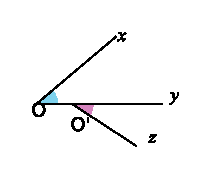
\includegraphics[width=.85\linewidth]{acti1} &
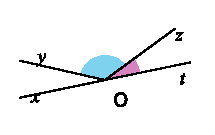
\includegraphics[width=.85\linewidth]{acti2} &
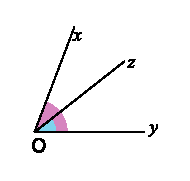
\includegraphics[width=.85\linewidth]{acti3} &
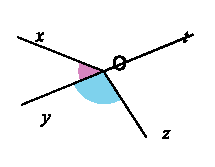
\includegraphics[width=.85\linewidth]{acti4} \\ 
\end{tabularx}

\begin{enumerate}
\item Dans les figures 2 et 4, les angles bleu et rose sont dits \textbf{adjacents}. Ce n'est pas le cas pour les autres figures. À partir de tes observations, essaie d'expliquer à quelles conditions deux angles sont adjacents. 
\item Deux angles adjacents ont-ils nécessairement la même mesure ? Justifie ta réponse.

\vspace{1em}

\begin{tabularx}{\linewidth}{XXXX}
\multicolumn{1}{c}{Figure 5} &
\multicolumn{1}{c}{Figure 6} &
\multicolumn{1}{c}{Figure 7} &
\multicolumn{1}{c}{Figure 8} \\
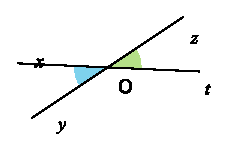
\includegraphics[width=.85\linewidth]{acti5} &
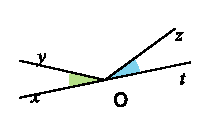
\includegraphics[width=.85\linewidth]{acti6} &
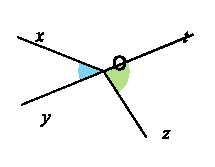
\includegraphics[width=.85\linewidth]{acti7} &
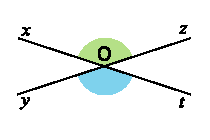
\includegraphics[width=.85\linewidth]{acti8} \\ 
\end{tabularx}

\item Dans les figures 5 et 8, les angles bleu et vert sont dits \textbf{opposés par le sommet}. Ce n'est pas le cas pour les autres figures. À partir de tes observations, essaie d'expliquer à quelles conditions deux angles sont opposés par le sommet.
\item Deux angles opposés par le sommet ont-ils nécessairement la même mesure ? Justifie ta réponse en utilisant une propriété sur deux angles symétriques par rapport à un point.
\end{enumerate}
\end{activite}


\begin{activite}[De jolies sommes !]
\begin{enumerate} \item Trace un triangle $ABC$ rectangle en $A$ puis mesure les angles $\widehat{ABC}$ et $\widehat{BCA}$.
\item Marie affirme que tous les élèves de la classe ne trouveront pas nécessairement les mêmes mesures mais qu'il y a quand même une relation entre ces deux mesures. Quelle est-elle ? Justifie ta réponse.

\vspace{1em}

On dit que deux angles sont \textbf{complémentaires} lorsque la somme de leurs mesures est égale à 90°. 
\item Les angles $\widehat{ABC}$ et $\widehat{BCA}$ sont-ils complémentaires ?
\item  Construis deux angles complémentaires \textbf{et} adjacents dont l'un mesure 64°.
\item Ahmed a mesuré l'angle $\widehat{xOz}$ ci-dessous et a trouvé 110°.

\begin{center}
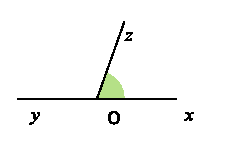
\includegraphics[width=.25\linewidth]{acti9}
\end{center}

Sa voisine lui dit que ce n'est pas possible et qu'à partir de l'erreur d'Ahmed elle pense connaître la bonne mesure. Quelle est cette mesure ? Comment a-t-elle pu la trouver ?

\vspace{1em}

On dit que deux angles sont \textbf{supplémentaires} lorsque la somme de leurs mesures est égale à 180°. 
\item Les angles $\widehat{xOz}$ et $\widehat{zOy}$ sont-ils supplémentaires ?
\item Construis deux angles supplémentaires \textbf{et} non adjacents dont l'un mesure 52°.
\end{enumerate}
\end{activite}


\begin{activite}[Avec des angles correspondants égaux...]
\begin{enumerate}
\item Observe la figure ci-dessous puis reproduis-la en choisissant la même mesure pour les angles $\widehat{ERF}$ et $\widehat{ESH}$.

\begin{center}
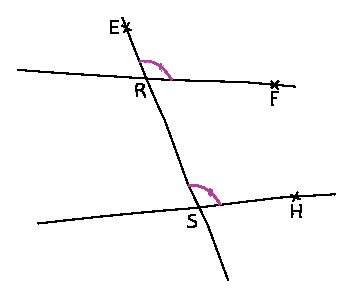
\includegraphics[width=.25\linewidth]{acti10}
\end{center}

\item\label{AactiquestionAngles} Comment peux-tu qualifier les angles $\widehat{ERF}$ et $\widehat{ESH}$ ? 
\item\label{AactiquestionDroites} Sur ta figure, quelle est la position relative des droites $(RF)$ et $(SH)$ ?
\item\label{AactiquestionPhrase} À l'aide des questions \ref{AactiquestionAngles} et \ref{AactiquestionDroites}, recopie puis complète la phrase : \textsl{« Si deux angles correspondants sont ... alors les deux droites coupées par la sécante sont ... . »}.
\item Écris une propriété identique à celle de la question \ref{AactiquestionPhrase} pour les angles alternes-internes.
\end{enumerate}
\end{activite}